\documentclass{article}
%\documentclass{standalone}

\usepackage{biblatex} 

\usepackage{tikz}

\begin{document}

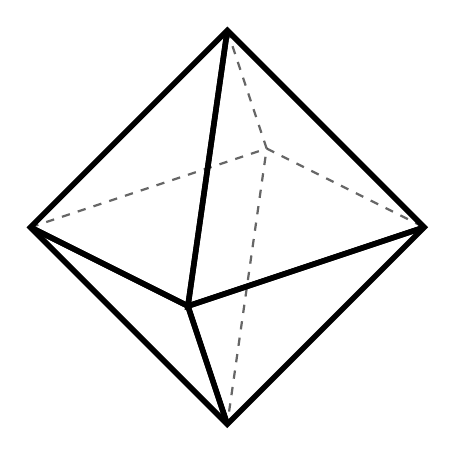
\begin{tikzpicture}[thick,scale=5]

\coordinate (A1) at (0,0);
\coordinate (A2) at (0.6,0.2);
\coordinate (A3) at (1,0);
\coordinate (A4) at (0.4,-0.2);
\coordinate (B1) at (0.5,0.5);
\coordinate (B2) at (0.5,-0.5);

\begin{scope}[thick,dashed,,opacity=0.6]
\draw (A1) -- (A2) -- (A3);
\draw (B1) -- (A2) -- (B2);
\end{scope}
\draw[solid][line width=2pt] (A1) -- (A4) -- (B1);
\draw[solid][line width=2pt] (A1) -- (A4) -- (B2);
\draw[solid][line width=2pt] (A3) -- (A4) -- (B1);
\draw[solid][line width=2pt] (A3) -- (A4) -- (B2);
\draw[solid][line width=2pt] (B1) -- (A1) -- (B2) -- (A3) --cycle;

\end{tikzpicture}

%\begin{tikzpicture}[thick,scale=5]
%
%\coordinate (C1) at (0.2,0);
%\coordinate (C2) at (0.8,-0.1);
%
%\begin{scope}[thick,dashed,,opacity=0.6]
%\draw (C1) -- (C2);
%
%\end{scope}
%\draw[solid][line width=2pt] (C1) -- (A4) -- (B1);
%\draw[solid][line width=2pt] (C1) -- (A4) -- (B2);
%\draw[solid][line width=2pt] (C2) -- (A4) -- (B1);
%\draw[solid][line width=2pt] (C2) -- (A4) -- (B2);
%\draw[solid][line width=2pt] (B1) -- (C1) -- (B2) -- (C2) --cycle;
%
%\end{tikzpicture}

\vspace{3cm}
\centering
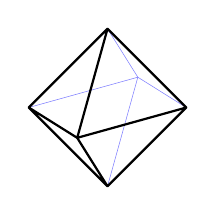
\begin{tikzpicture}[line cap=round,line join=round]
  \path
  ( 1, 0, 0) coordinate (A1)
  ( 0, 0,-1) coordinate (A2)
  (-1, 0, 0) coordinate (A3)
  ( 0, 0, 1) coordinate (A4)
  ( 0, 1, 0) coordinate (B1)
  ( 0,-1, 0) coordinate (B2);

  \begin{scope}[very thin,draw=blue!50]
    \draw
    (A1) -- (A2) -- (A3)
    (B1) -- (A2) -- (B2);
  \end{scope}

  \draw[thick]
  (A1) -- (A4) -- (B1)
  (A1) -- (A4) -- (B2)
  (A3) -- (A4) -- (B1)
  (A3) -- (A4) -- (B2)
  (B1) -- (A1) -- (B2) -- (A3) --cycle;
\end{tikzpicture}

\vspace{3cm}


% DEFINING COLORS COF, PUR, GREEO AND GREET
\definecolor{cof}{RGB}{219,144,71}
\definecolor{pur}{RGB}{186,146,162}
\definecolor{greeo}{RGB}{91,173,69}
\definecolor{greet}{RGB}{52,111,72}
% OCTAHEDRON
\begin{tikzpicture}[thick,scale=3]
    \coordinate (A1) at (0,0);
    \coordinate (A2) at (0.6,0.2);
    \coordinate (A3) at (1,0);
    \coordinate (A4) at (0.4,-0.2);
    \coordinate (B1) at (0.5,0.5);
    \coordinate (B2) at (0.5,-0.5);
    %
    \begin{scope}[thick,dashed,,opacity=0.6]
        \draw (A1) -- (A2) -- (A3);
        \draw (B1) -- (A2) -- (B2);
    \end{scope}
    %
    \draw[fill=cof,opacity=0.6] (A1) -- (A4) -- (B1);
    \draw[fill=pur,opacity=0.6] (A1) -- (A4) -- (B2);
    \draw[fill=greeo,opacity=0.6] (A3) -- (A4) -- (B1);
    \draw[fill=greet,opacity=0.6] (A3) -- (A4) -- (B2);
    \draw (B1) -- (A1) -- (B2) -- (A3) --cycle;
\end{tikzpicture}


%% Bi-pyramid
%\begin{tikzpicture}[thick,scale=3]
%    \coordinate (A1) at (0,0);
%    \coordinate (A3) at (1,0);
%    \coordinate (A4) at (0.4,-0.2);
%    \coordinate (B1) at (0.5,0.5);
%    \coordinate (B2) at (0.5,-0.5);
%    %
%    \begin{scope}[thick,dashed,,opacity=0.6]
%        \draw (A1)  -- (A3);
%    \end{scope}
%    \draw[fill=cof,opacity=0.6] (A1) -- (A4) -- (B1);
%    \draw[fill=pur,opacity=0.6] (A1) -- (A4) -- (B2);
%    \draw[fill=greeo,opacity=0.6] (A3) -- (A4) -- (B1);
%    \draw[fill=greet,opacity=0.6] (A3) -- (A4) -- (B2);
%    %
%    \draw (B1) -- (A1) -- (B2) -- (A3) --cycle;
%    %
%\end{tikzpicture}


\printbibliography
\end{document}